%%%%%%%%%%%%%%%%%%%%%%%%%%%%%%%% 
\section{The Charge Readout System} 
\label{sec:detectors-fd-alt-chg-readout}

In the dual-phase LArTPC concept, the ionization charge is first
extracted into the argon gas phase using a 2-kV/cm electric field
defined across the liquid-gas interface with a submersed extraction
grid (stainless steel wires tensioned in both $x$ and $y$
directions). Once in the gas, the charge is amplified by the Large
Electron Multipliers (LEM). These are printed circuit boards with
conductive layers (electrodes) on the two sides and many holes drilled,
through.  By applying voltages across the two
electrodes a 30-kV/cm electric field region is defined in the holes
of the micro pattern structure of the LEM\cite{Bondar:2008yw}. Electrons
transiting through the holes trigger Townsend multiplication in the
pure gas Argon contained in these high electric field regions.

The amplified charge is then collected and recorded on a 2D anode
consisting of two sets of 3.125-mm-pitch strips that provide the $x$
and $y$ coordinates (and thus two views) of the event.

Typical electric fields between each stage of the readout are
illustrated in Figure~\ref{fig:setup}. Table~\ref{tab:crp_dist} shows
the inter-stage distance and the tolerances required to obtain
uniformity of gain to within $\sim$5\%.
\begin{cdrfigure}[Dual-phase readout]{setup}{Illustration of the electric fields in the amplification region of a dual-phase LArTPC. The simulated field lines in dark blue indicate the paths followed by the drifting charges (without diffusion).}
 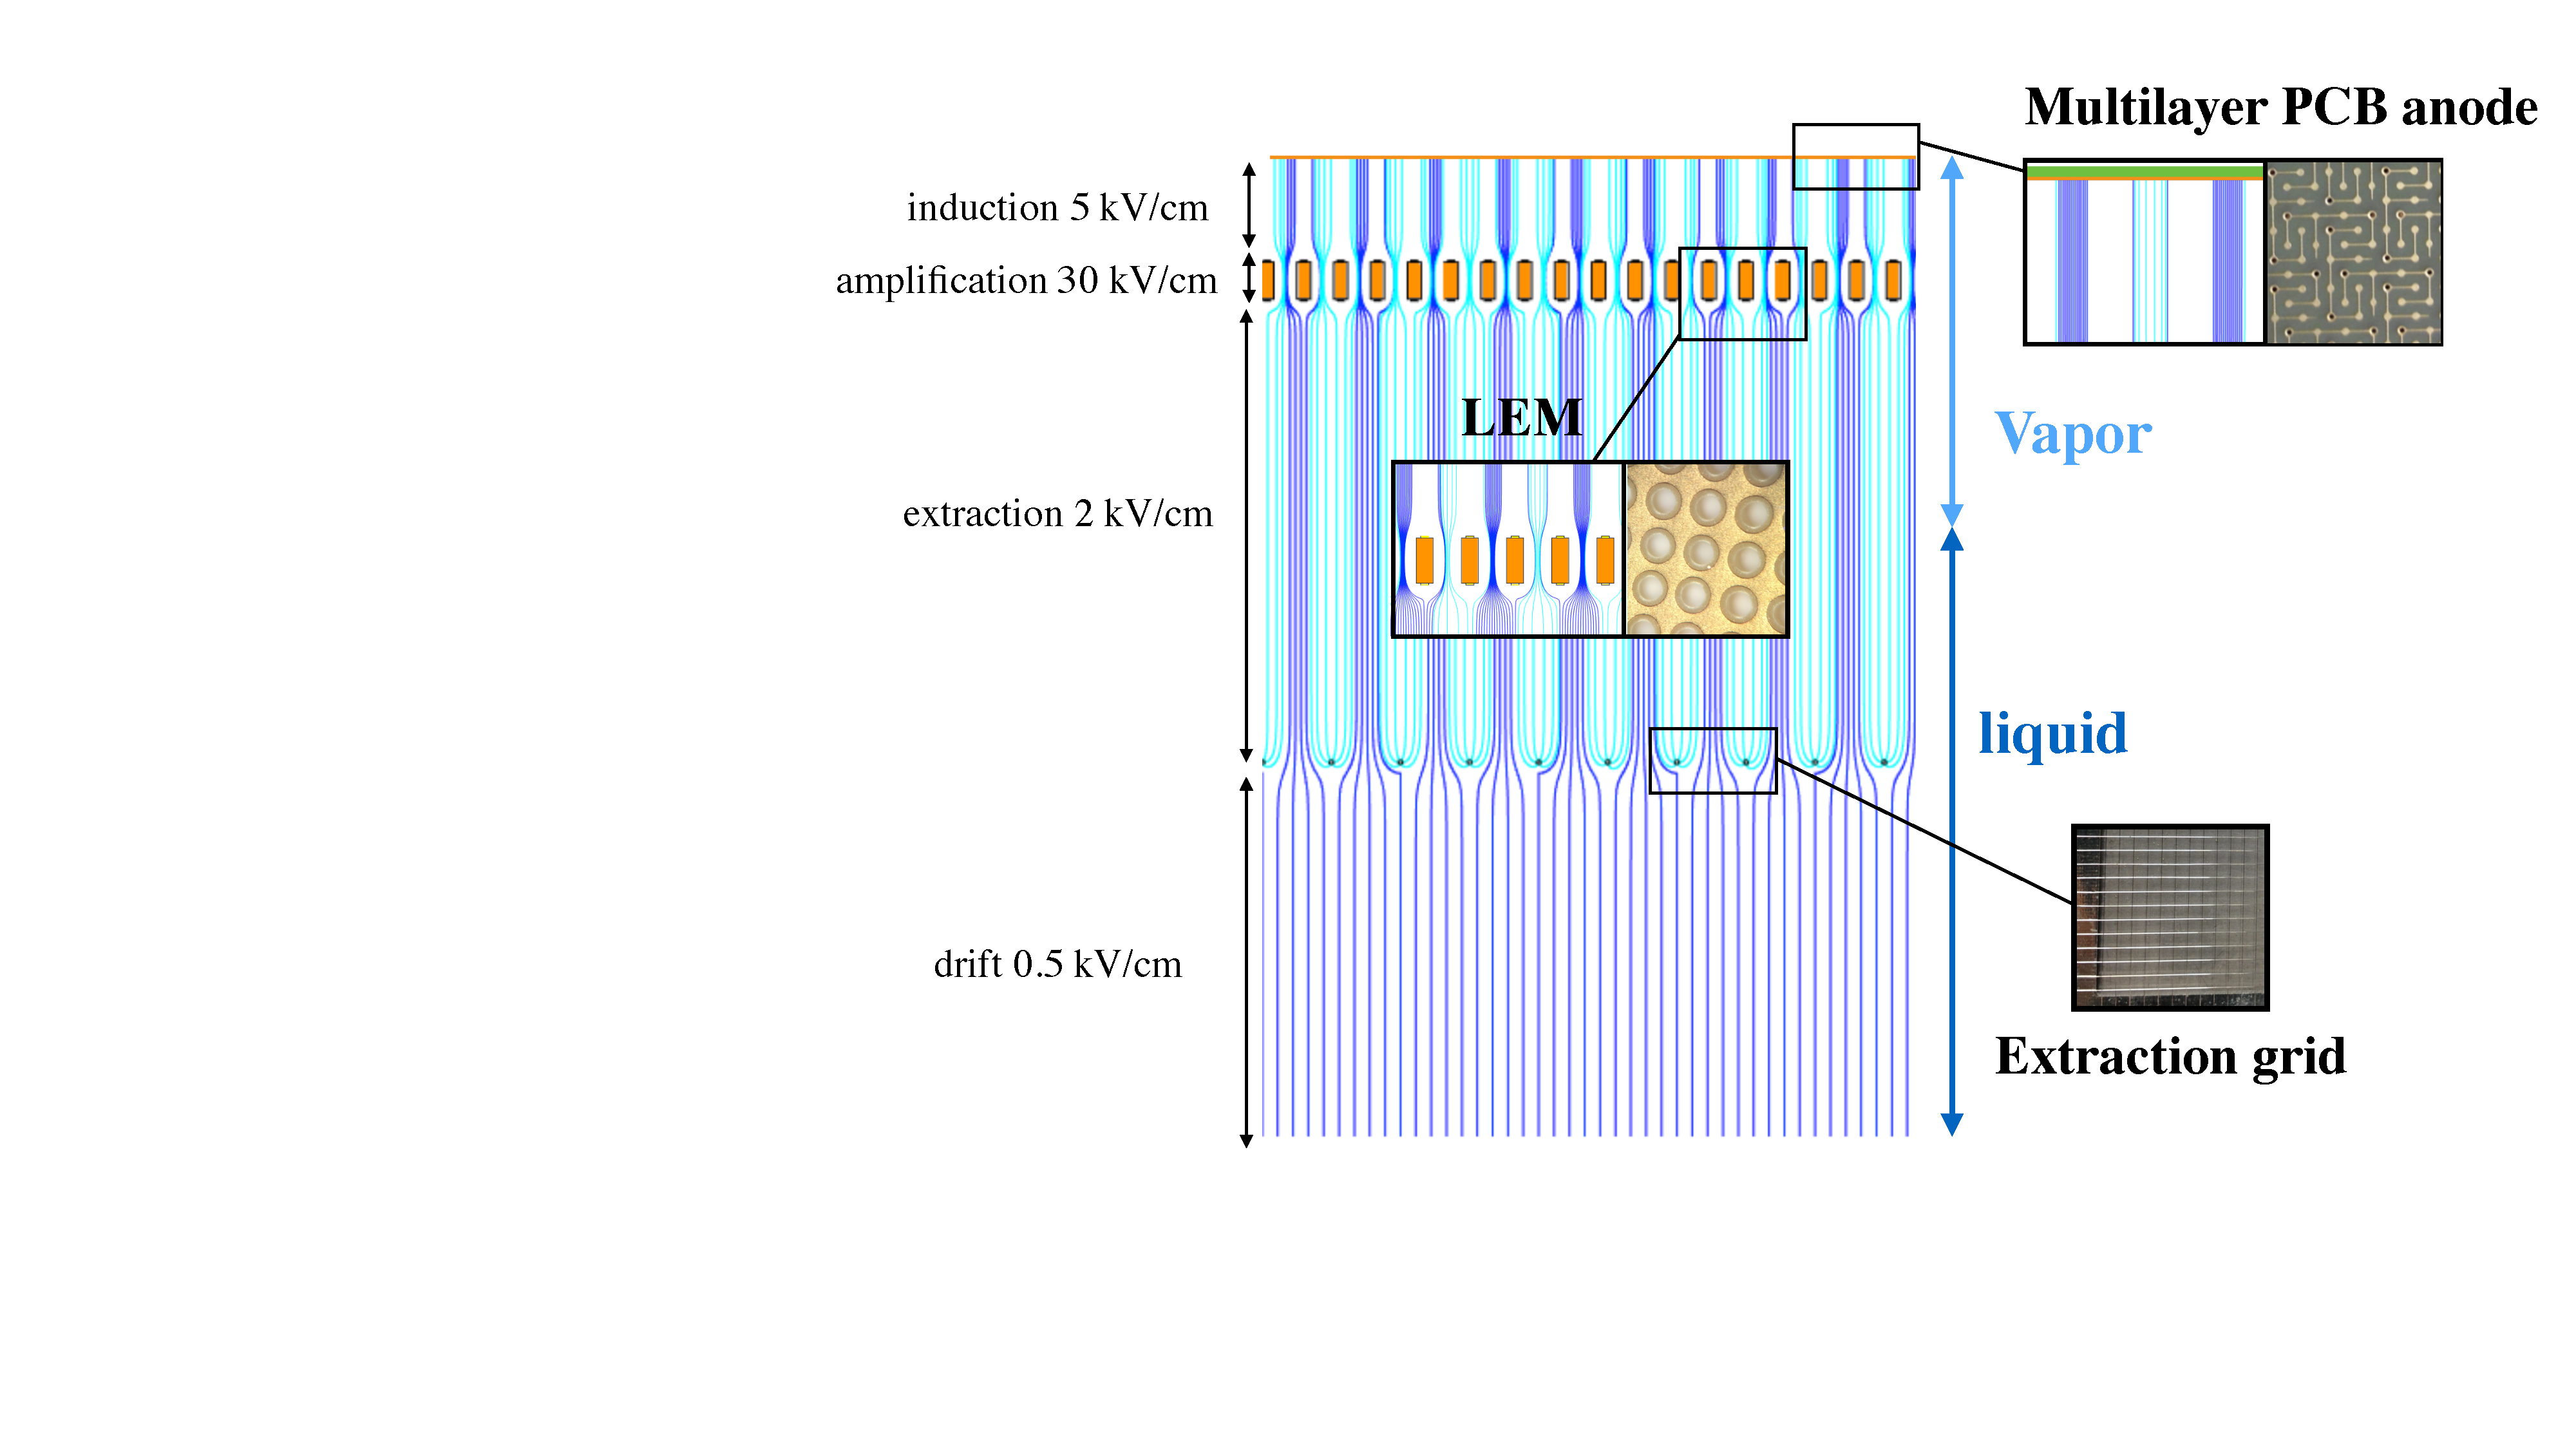
\includegraphics[width=.8\textwidth]{double_phase_principle.pdf}  
\end{cdrfigure}
\begin{cdrtable}[Interstage distances and electric field settings of the dual-phase readout components]{lp{2cm}p{2cm}l}{crp_dist}{Interstage distances and electric field settings of the dual-phase readout components.} 
 Component & Distance [mm] & Tolerance [mm] & Electric field [kV/cm]  \\ \toprowrule
 Anode-LEM top electrode  & 2 & 0.1 & 5\\ \colhline
 LEM top-bottom electrode   & 1 & 0.01 & 30-35\\ \colhline
 LEM bottom electrode-grid        & 10 & 1 & 2 (in LAr) and 3 (in GAr)\\
 \end{cdrtable}

The three stages (extraction grid, LEM and anode) are assembled into
multi-layered, sandwich-like modular units (\num{9}m$^2$ in area) with
precisely defined inter-stage distances and inter-alignment; these
modular units are called Charge Readout Planes (CRPs).
   
\subsection{The Charge Readout Plane (CRP)}

Each CRP is an independent detector element that performs charge
extraction, multiplication and collection, and has its own high
voltage system and independent signal feedthroughs. The entire area of
the LEM and anode in a CRP is active.

The LBNO 20-kt detector design (described in \anxlbnob) featured
modularized CRPs of dimensions of 4$\times$4~m$^2$, with 2-m long
strips. For the DUNE cryostat geometry, a size of 3$\times$3~m$^2$
with a strip length of 3~m is found to be optimal. The description in
this section is based on the LBNO 4$\times$4~m$^2$ CRP.

The LEM and anode pre-mounted units of 50$\times$50~cm$^2$, called
LEM/Anode Sandwich (LAS) modules, are assembled into a CRP. Each LAS
anode is segmented in 50-cm long X and Y strips . Adjacent LAS anodes
are bridged together to form readout strips of the required length by
connecting short flat cables to KEL connectors soldered on the top
sides of the anodes. The signals from the last anode forming the
strips chain are brought with 50-cm long flat cables to feedthoughs
mounting on the other side the front-end electronics embedded inside
dedicated signal-feedthrough chimneys.

Each CRP is independently hung from the vessel deck through its three
suspension feedthroughs and has its own high voltage system and its
independent signal and slow control feedthroughs.
Figure~\ref{fig:4_4CRP_FRONT} illustrates the 4$\times$4 m$^2$ CRP;
its characteristics are summarized in Table~\ref{tab:crp_para}.
\begin{cdrfigure}[Side and top views of the $4\times4$~m$^2$ CRP]{4_4CRP_FRONT}{Side and top views of the $4\times4$~m$^2$ CRP designed for LBNO (units in mm).}
 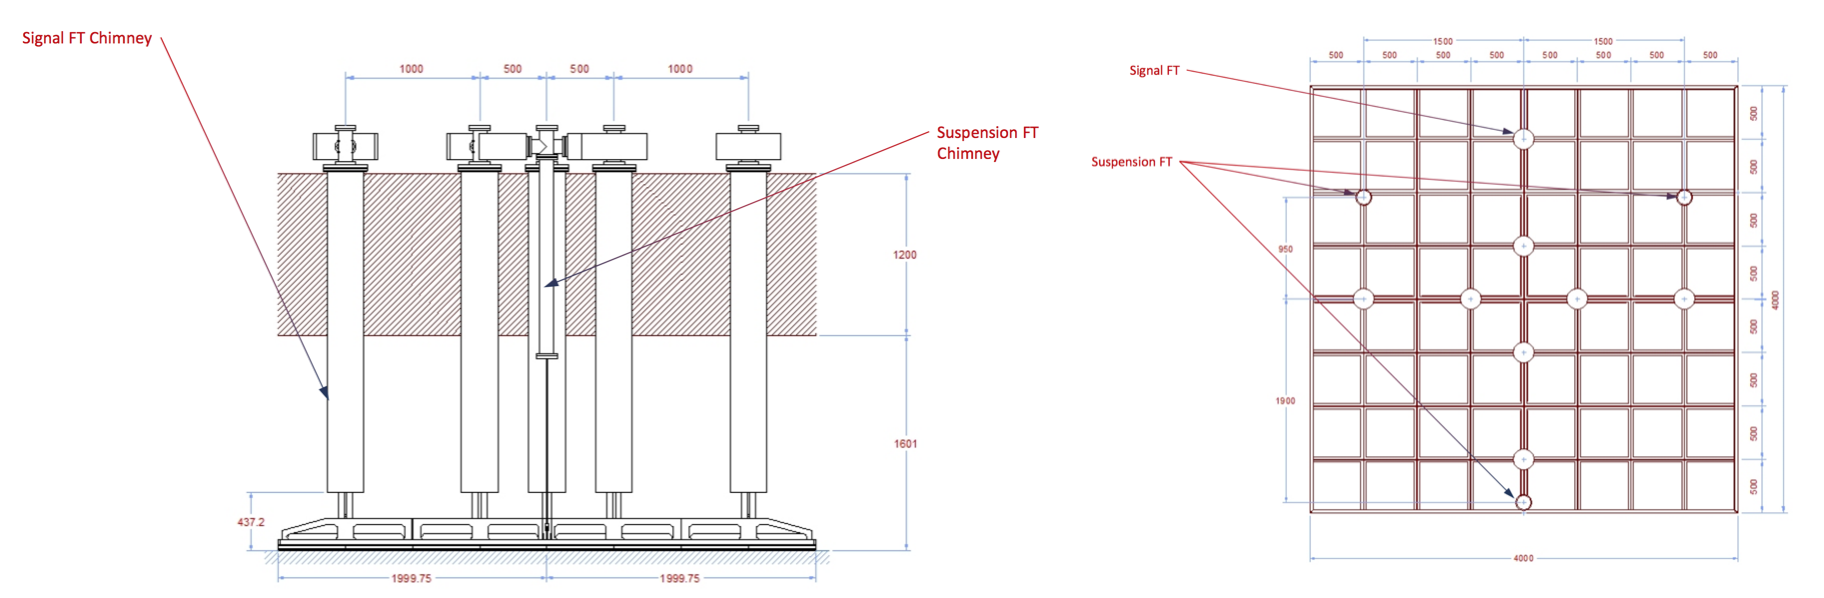
\includegraphics[width=\textwidth]{4_4_CRP_top-side-view}  
\end{cdrfigure}
\begin{cdrtable}[Numbers of components of the 4$\times$4 m$^2$ CRP]{lr}{crp_para}{Numbers of components of the 4$\times$4 m$^2$ CRP designed for LBNO} 
Component & Number \\ \toprowrule
$50\times50$ cm$^2$ anode panels & 64\\ \colhline
$50\times50$ cm$^2$ LEM  panels&  64\\ \colhline
Signal  feedthroughs & 8\\ \colhline
Suspension  feedthroughs & 3\\ \colhline
Readout strip length (m)& 2\\ \colhline
Number of channels & 5120\\
\end{cdrtable}

The entire area of the LEM and anode is active, as noted earlier, and
each adjacent 50$\times$50~cm$^2$ LAS module has a gap of only 0.5~mm.
Therefore, the entire 4$\times$4~m$^2$ area of the CRP is fully
active, with a small gap every 50~cm that does not interfere with the
charge collection in the 3.125-mm readout pitch of the anode.

The extraction grid consists of 100~$\mu$m diameter stainless steel
wires tensioned in both $x$ and $y$ directions over the entire 4-m
length of the CRP. They are soldered into groups of 32 on independent
wire-tensioning pads oriented perpendicularly to the side of the CRP
frame.  Each wire-tensioning pad consists of a printed circuit board
(PCB) for HV-connection that is fixed to a mechanical wire holder very
precisely. The PCB has 32 soldering pads with 200~$\mu$m grooves for
precise positioning of the wires. During the wire-soldering process
each wire is tensioned by 150-g lead weights and positioned in a
groove.  (With this method better than 50~$\mu$m precision on the wire
pitch, measured under the microscope, was achieved for the LBNO-WA105
prototypes.) The PCB is then mounted on the wire holder and the
tension of the group f 32 wires can be precisely adjusted by pushing
the holder against the CRP's FR4 frame with two screws.


The 4$\times$4~m$^2$ CRP has 5120 readout channels in total. The
signals from the CRP are read out through eight signal feedthroughs
(SFTs) that host the front-end electronics at its bottom and transmit
the signal to the DAQ system located on top outside of the vessel.
Each signal feedthrough groups 640 channels. Three suspension
feedthroughs are arranged as an equilateral triangle whose barycenter
coincides with that of the CRP; they suspend the CRP at the required
position and precisely adjust the CRP level with respect to the liquid
argon surface. Figure~\ref{fig:4_4CRP_3D} shows a 3D view of this CRP,
where the chimneys for feedthroughs and the stiffening frame are
visible.
\begin{cdrfigure}[3D view of the $4\times4$~m$^2$ CRP.]{4_4CRP_3D}{3D view of the $4\times4$~m$^2$ LBNO CRP.}
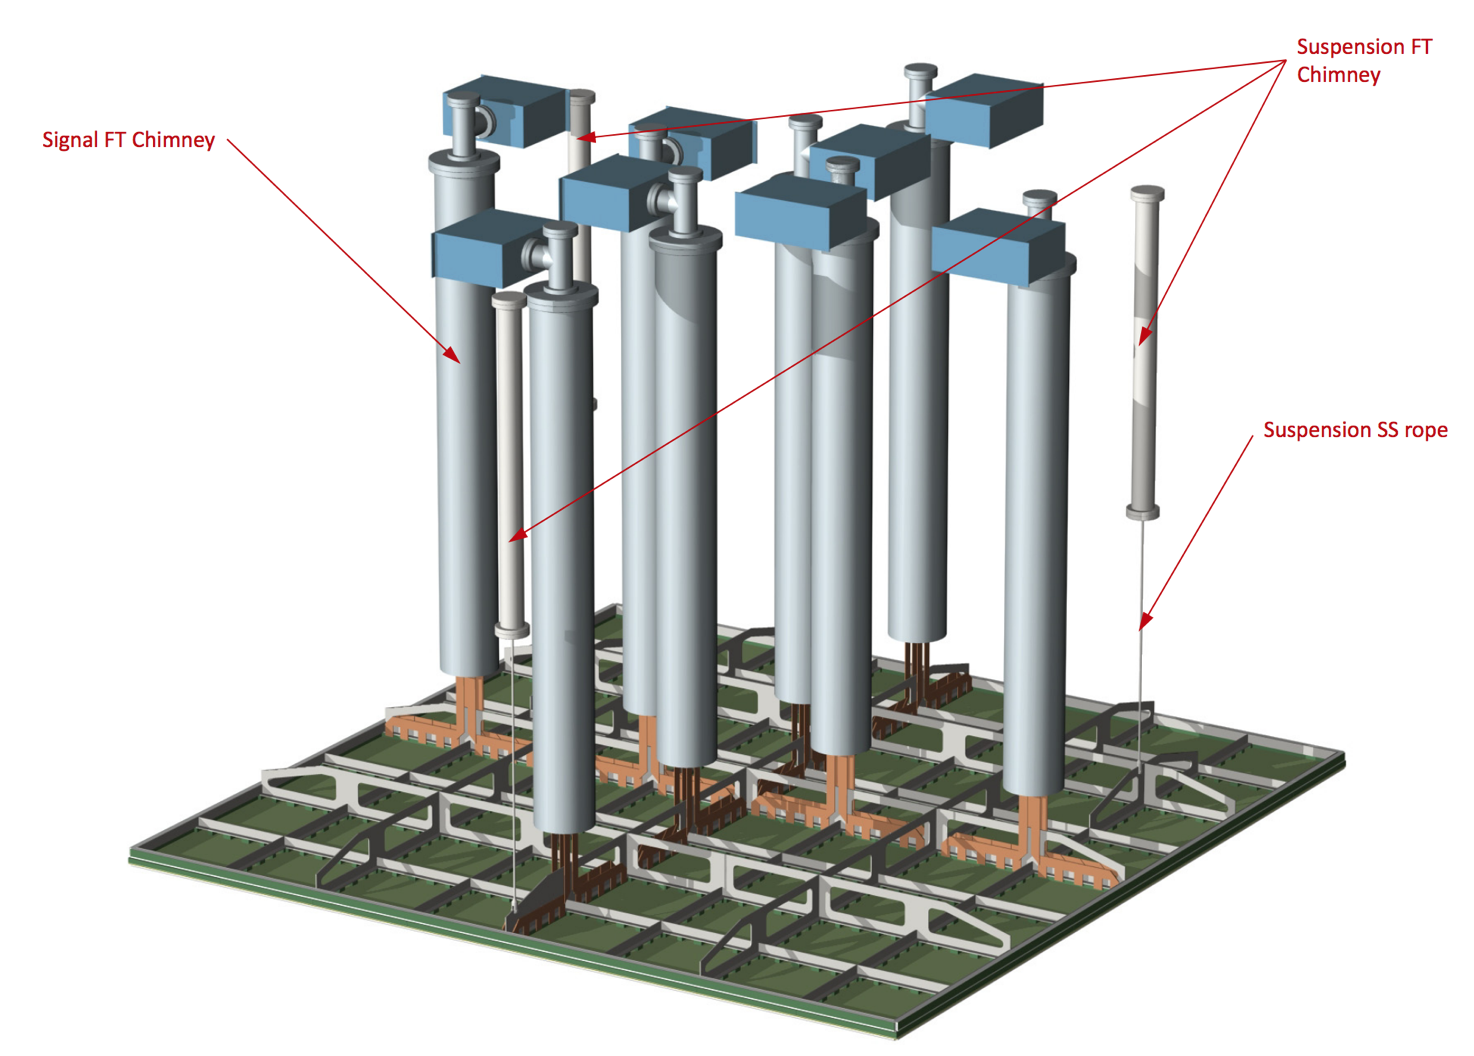
\includegraphics[width=0.8\textwidth]{4_4CRP_3D}  
\end{cdrfigure}

The 3$\times$3~m$^2$ DUNE CRP, is a down-sized version of the LBNO
CRP, it has three signal feedthrough chimneys and 1920 readout
channels.


%%%%%%%%%%%%%%%%%%%%%%%%%%%%%%%%%%%%%%%%%
\subsection{The LEM/Anode Sandwich (LAS)}

LAS modules have been extensively studied as part of the ongoing CERN
WA105 prototyping efforts (see~\ref{sec:proto-cern-double}). The LEMs
and the anodes are produced by a PCB manufacturing company called
ELTOS\footnote{\url{www.eltos.it}}. Their designs are the outcome of
intensive R\&D effort over the last few years, aimed at maximizing the
S/N ratio for the large-area readouts foreseen for use in giant
dual-phase LArTPCs.  Figure~\ref{fig:LEM_anode} shows the LEMs and
anodes.  This section summarizes key features of the LAS.
\begin{cdrfigure}[Pictures of the LEM and anode along with microscope views]
{LEM_anode}{Top: pictures of the LEM and anode along with microscope
  views. Bottom: close up of the LEM HV connectors and back view of the anode 
with the KEL signal connectors to bridge to the adjacent LAS or to connect 
flat cables going to the signal feedthrough}
 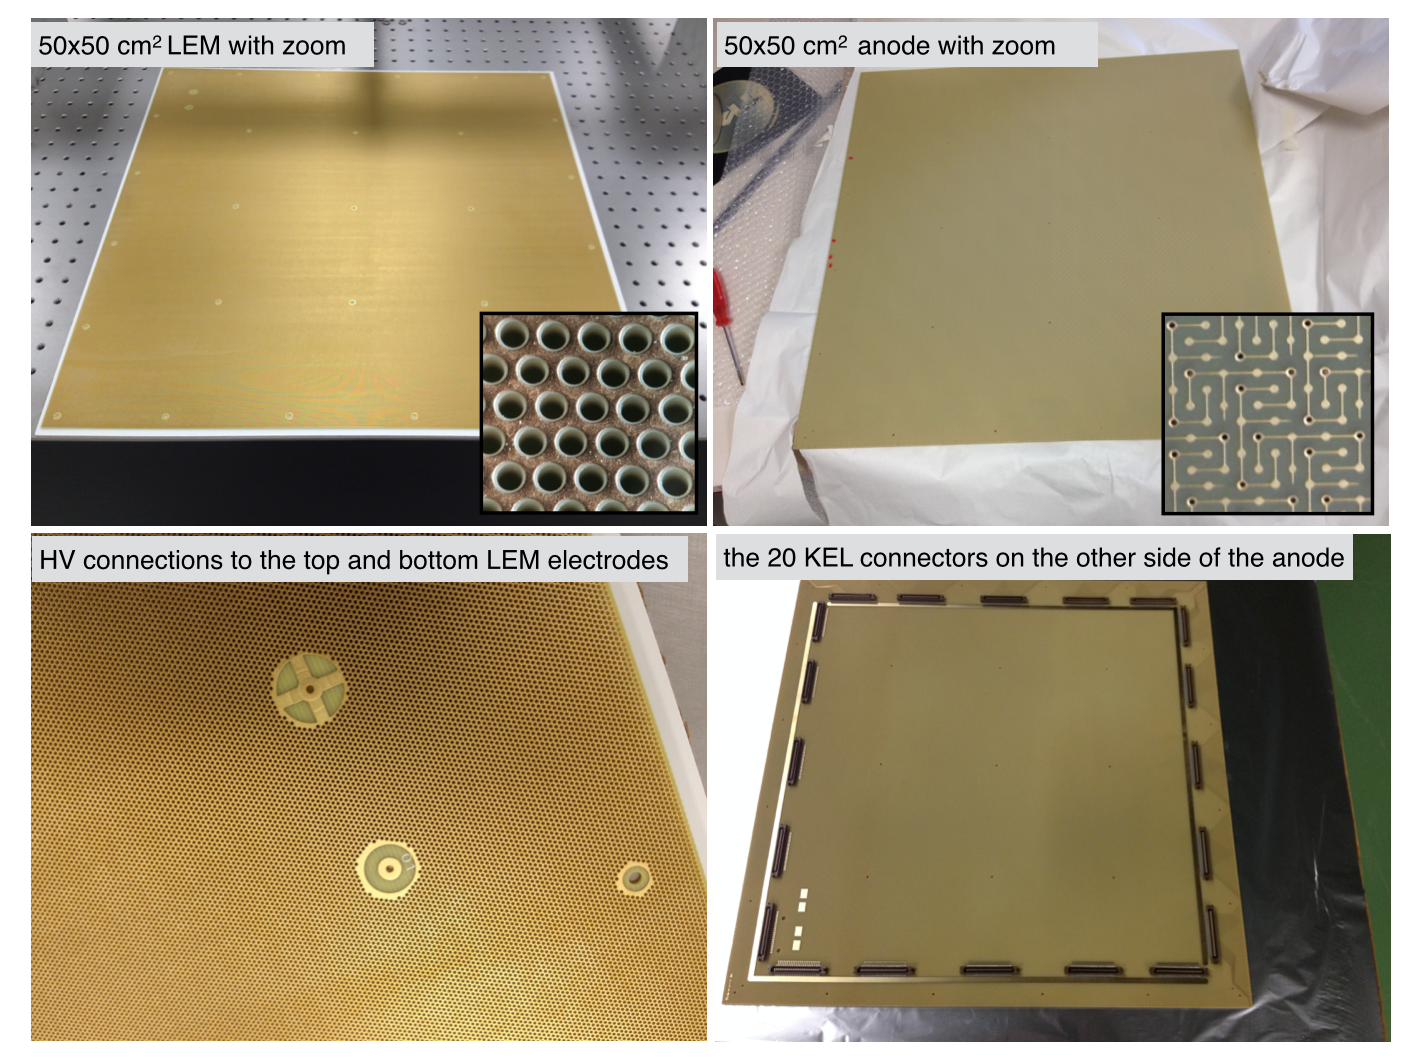
\includegraphics[width=.8\textwidth]{LEM_anode_zoom}  
 \end{cdrfigure}


 \paragraph{The 0.5$\times$0.5~m$^2$ anode:}

The anode is manufactured from a single multilayer Printed Circuit
Board (PCB). The readout strips for both $x$ and $y$ views consist of
interconnected gold-plated copper tracks, corresponding to the
3.125-mm readout pitch. The two views have superimposed track patterns
that are however electrically insulated. This is possible by ensuring
the electrical continuity of a track, when crossing the one of the
perpendicular view, on the bottom layer of the PCB with a system of
vias connecting the two layers.

The design of the track patterns is such that both $x$ and $y$ views
collect the same amount of charge, independent of the angle of
charged-particle tracks with respect to the readout strip
orientation. This design has been optimized by testing various PCB
layouts as described in\cite{Cantini:2013yba}.  The layout and
schematic of the anode are shown in Figure~\ref{fig:anode_sch}.
\begin{cdrfigure}[The 2D anode]{anode_sch}
{The 2D anode (left) and its schematic explaining the  interconnections 
between both views (right). One view is filled  in red and the other in white.}
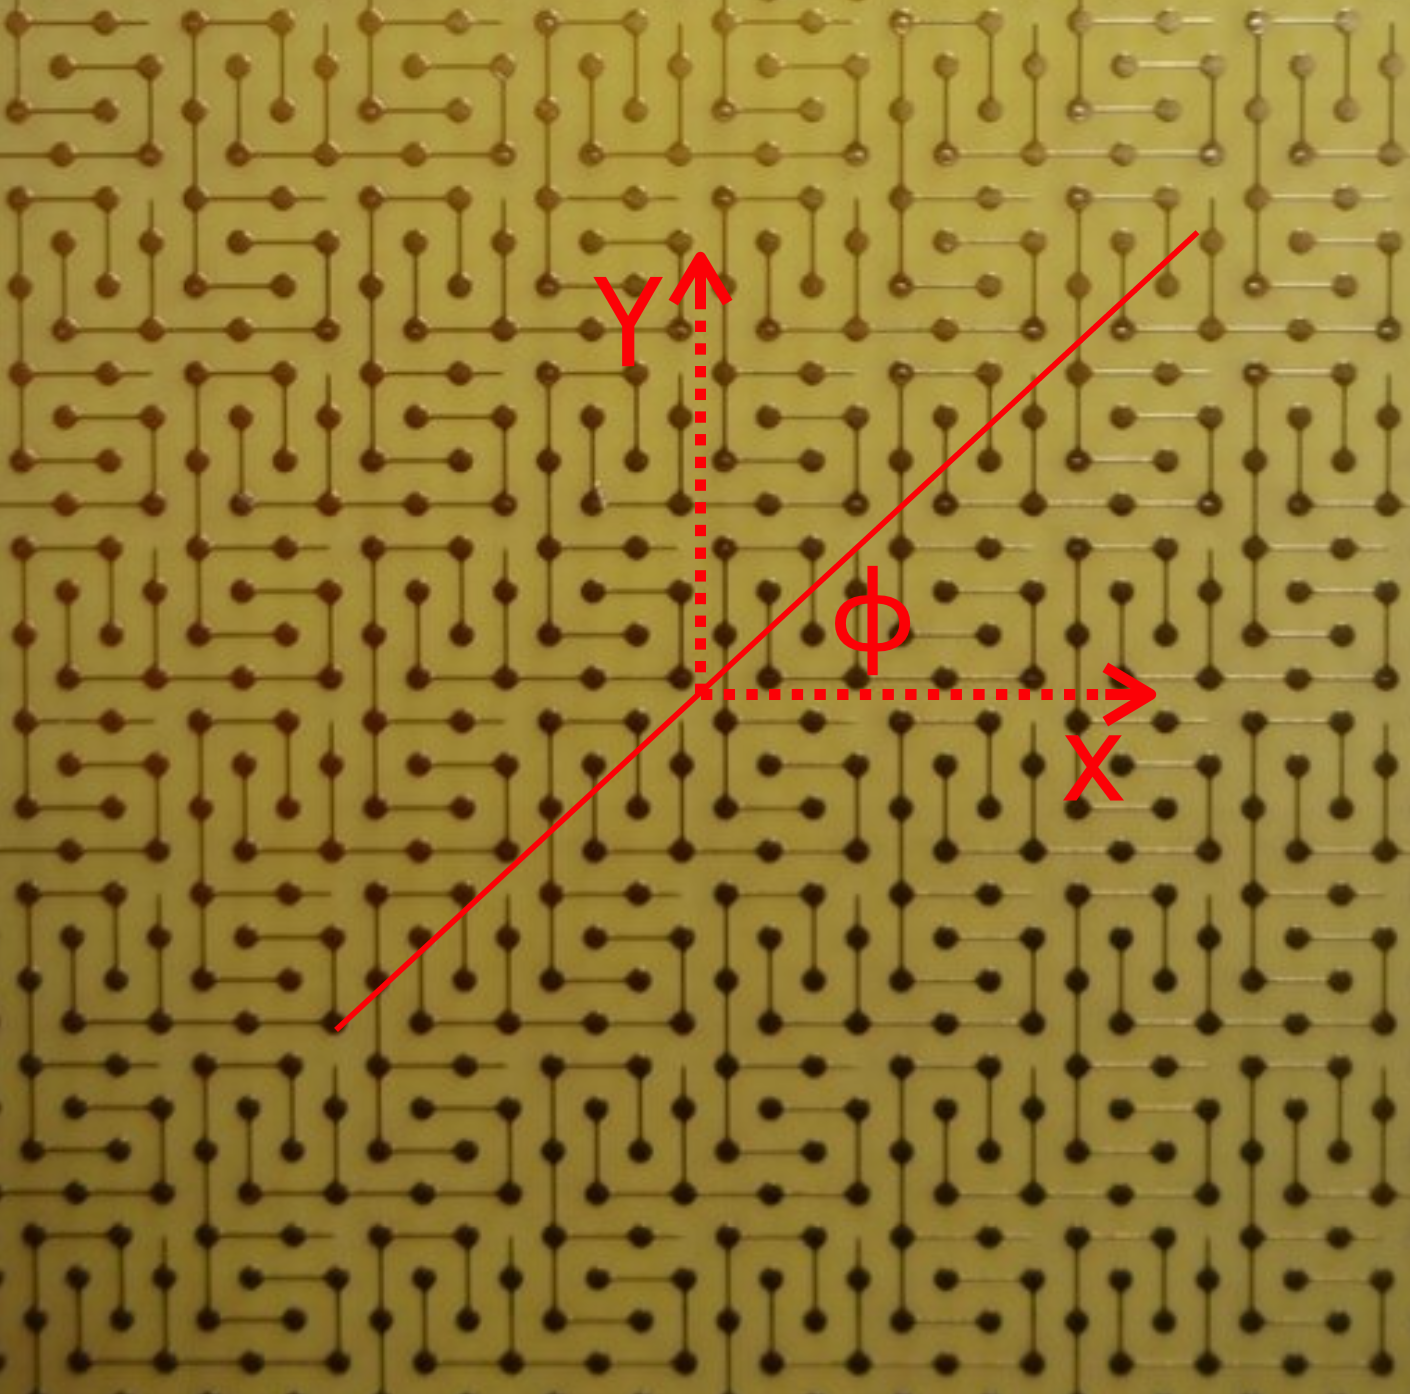
\includegraphics[scale=0.2]{anode_pcb} \hspace{0.2cm} 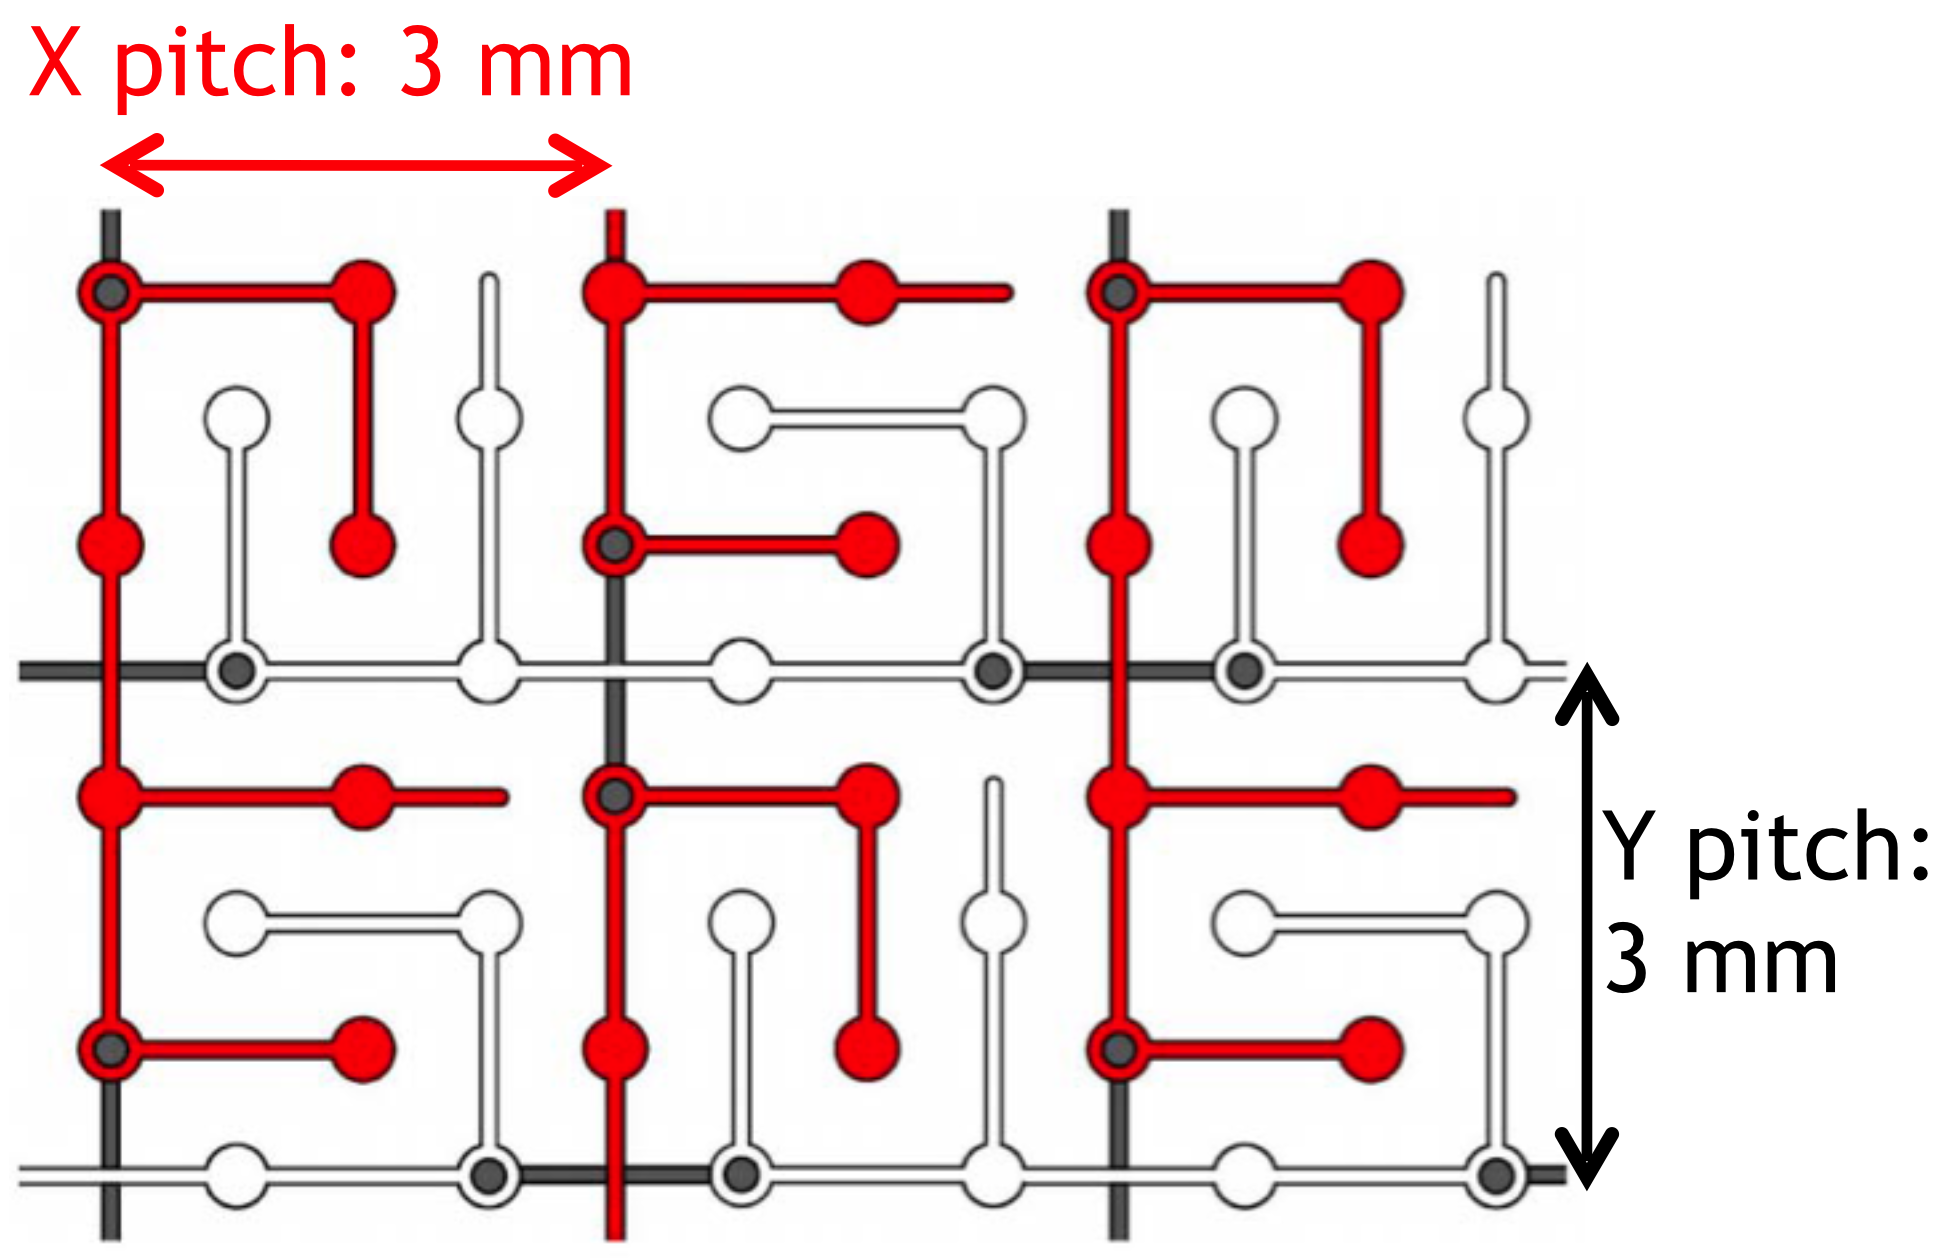
\includegraphics[scale=0.2]{anode_sch}
\end{cdrfigure}

As part of this optimization, the electrical capacitance of the
readout strips has been limited to only 150~pF/m, which translates
into an electronic noise of about $\sim$1000 electrons for 2-m readout
length.  Figure~\ref{fig:anode_res} (right) shows that the
charge-sharing asymmetry between the two views is kept within 1\%
. The two views can thus be treated in a completely equivalent way
from the point of view of the reconstruction. The response in terms of
the charge collection per unit pathlength $\Delta Q/\Delta s$ is
independent of the charged-particle tracks' azimuthal angle $\phi$
(see Figure~\ref{fig:anode_res} left and middle).
\begin{cdrfigure}[Charge deposition as function of track angle ]{anode_res} {Charge deposition per unit of pathlength measured on LEM view 0 
($\Delta Q_0/\Delta s_0$) as a function  of the track angle $\phi$ (left) and  projection of the  $\Delta Q_0/\Delta s_0$ distribution in three $\phi$ intervals (middle).  The right plot  shows the distribution of the difference between the total charge  collected on both views normalized to their sum}
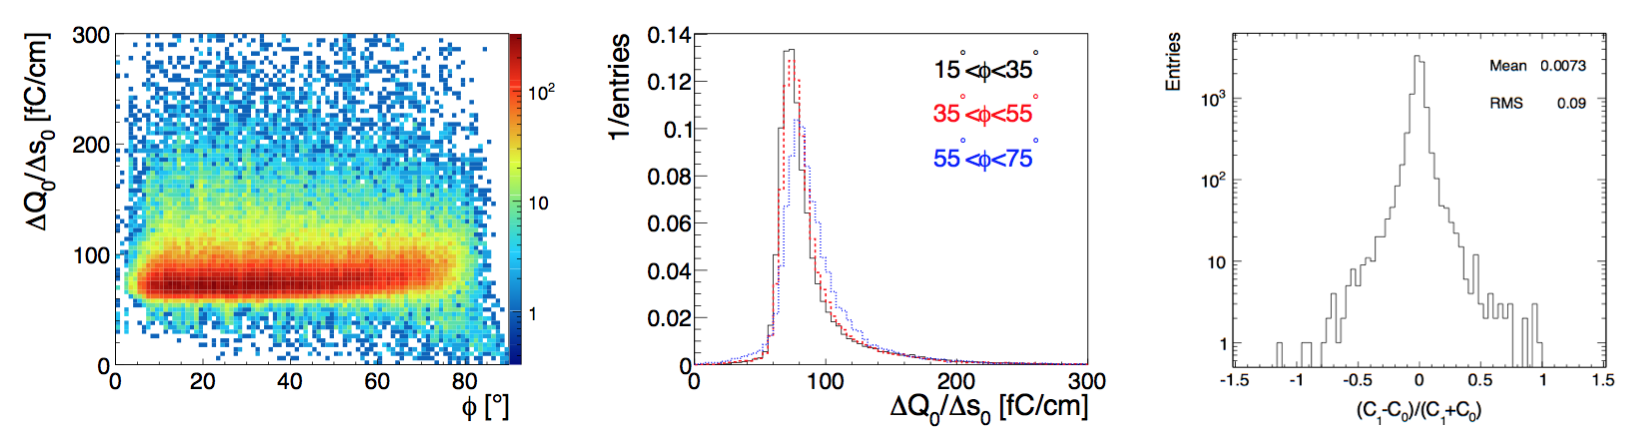
\includegraphics[width=.9\textwidth,scale=1]{anodeD_prop}
\end{cdrfigure}

\paragraph{The 0.5$\times$0.5~m$^2$ LEM:}

The LEM is built from a 1-mm thick copper-clad epoxy PCB with
500~$\mu$m diameter holes drilled through surrounded by a
40-$\mu$m dielectric rim. The holes are arranged in a honeycomb
pattern with a pitch of 800~$\mu$m resulting in about 200 holes per
cm$^2$ and $\cal O$(500,000) holes over the entire 50$\times$50~cm$^2$
area. The holes provide confinement for the UV photons produced during
the avalanche process and thus act as a mechanical quencher to prevent
photon feedback. This property makes the LEM suitable for operation in
ultra-pure argon vapor without the addition of a quenching gas. The
amplification of the drifting charges in pure argon vapor at 87~K with
LEMs has been extensively demonstrated on a chamber with
10$\times$10~cm$^2$ area readout (see e.g.,
References\cite{Badertscher:2008rf,Badertscher:2010fi}) as well as on
a larger device consisting of a 40$\times$80~cm$^2$
readout\cite{Badertscher:2013wm}.  Both setups were successfully and
stably operated at constant gains of at least 15, corresponding to
S/N$\approx$60 for MIPs. Recent studies\cite{Cantini:2014xza}
characterize systematically the impact of the rim size, insulator
thickness, hole diameter and hole layout on 10$\times$10~cm$^2$ area
LEMs. The response in terms of maximal reachable gain and influence on
the collected charge uniformity as well as the long-term stability of
the gain has been thoroughly compared for these different
layouts. Some results are shown in Figure~\ref{fig:LEM}.  Gains of
almost 200 were reached and the LEMs could be operated at stable gains
of at least $\sim$15 after a charging up period of about a day.
\begin{cdrfigure}[LEM performance vs geometry]{LEM}{Performance of the LEMs with different geometry parameters. Left: effective gain vs. LEM electric field; right: the stabilizations of the effective gain over time.}
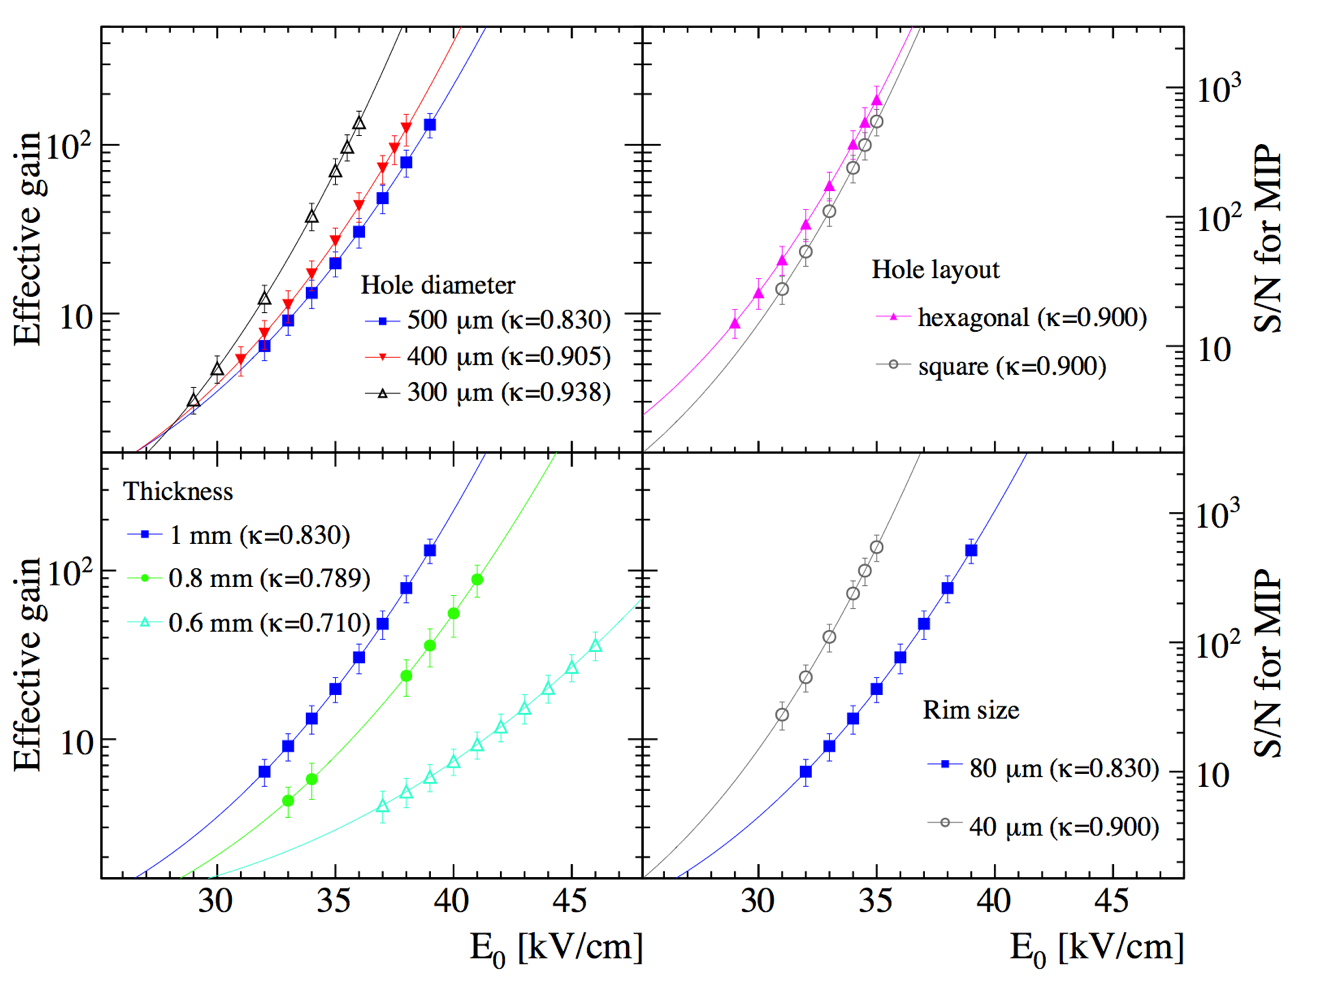
\includegraphics[scale=0.35]{4}
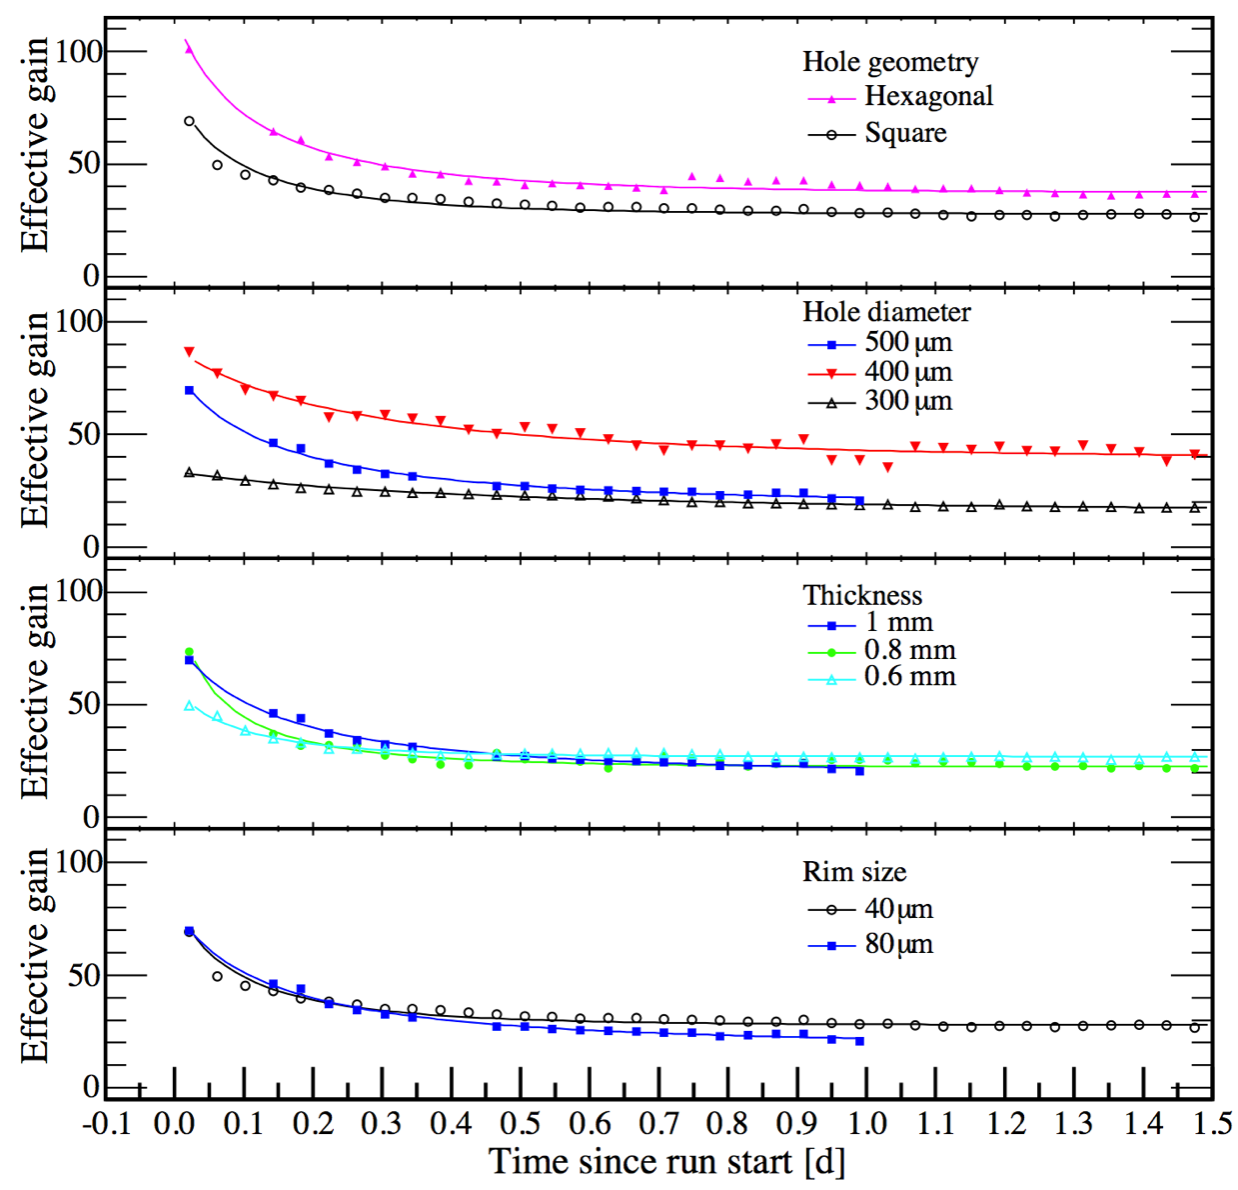
\includegraphics[scale=0.32]{3}
\end{cdrfigure}

\paragraph{LAS Assembly:}

Figure~\ref{fig:LEM_metro} shows the anode and LEM sandwich.  They are
fixed together with 29 M2 PEEK screws, each containing a precisely
machined 2-mm thick pillar to guarantee a constant inter-stage
distance between LEM and the anode on the entire $50\times50$~cm$^2$
area.  The dead zones caused by the supporting pillars and the two HV
pins on the LEMs are minimized and make up less than 0.5\% of the
total area. The inter-stage distance between the LEM and anode in the
LAS has been measured at many points. The results are shown in
Figure~\ref{fig:LEM_metro} and are described
in\cite{EDMS_metro_lem_anode}. They indicate that the planarity is
within the required tolerance of 2~mm$\pm$100~$\mu$m .
\begin{cdrfigure}[LEM/anode sandwich metrology]{LEM_metro}{Close up pictures of the LEM/anode sandwich. The two
       bottom figures show a the measurement at the CERN metrology lab
       and a histogram illustrating the measured gap between the LEM
       and anode in various points. As can be seen the distribution is
       centered on the nominal distance of 2~mm and has an RMS of
       about 100$\mu$m.}
     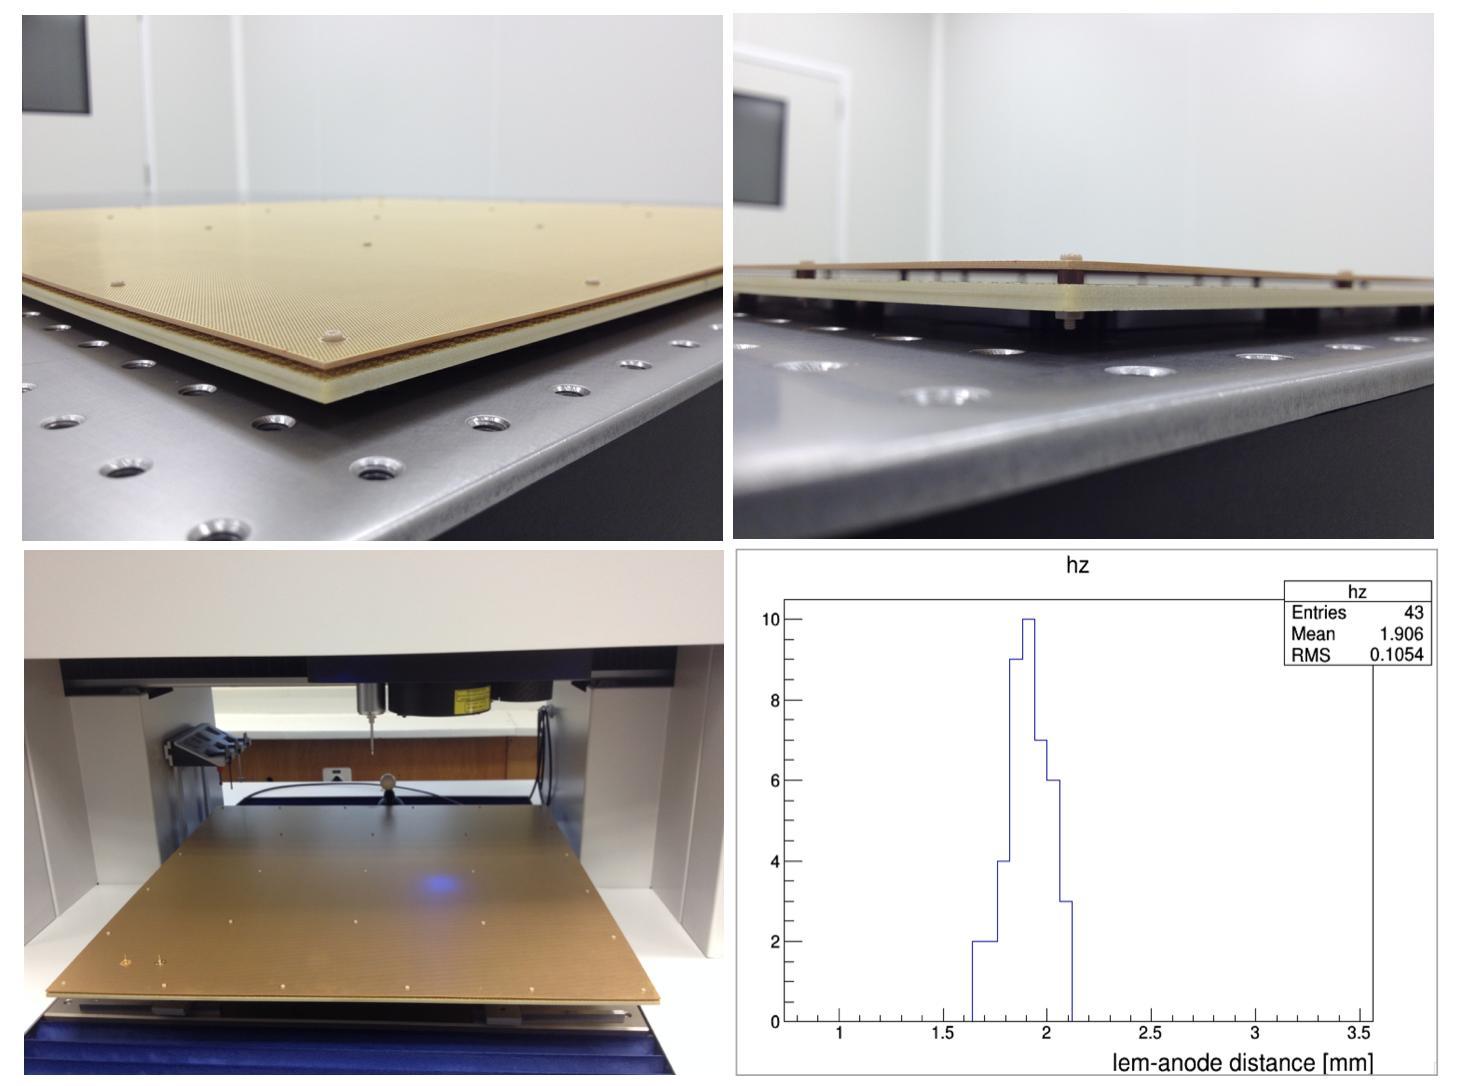
\includegraphics[width=.7\textwidth]{LEM_metro}
\end{cdrfigure}

The entire mounting sequence of the sandwich as well as that of the
different elements of the CRP are being addressed in the WA105
prototype detectors. An example of a sandwich assembly on a
$3\times1$~m$^2$ CRP is shown in Figure~\ref{fig:CRP_assembly}.
\begin{cdrfigure}[Pictures of the assembly of a $3\times1$m$^2$ CRP]{CRP_assembly}{Pictures of the assembly of a $3\times1$m$^2$ CRP}
     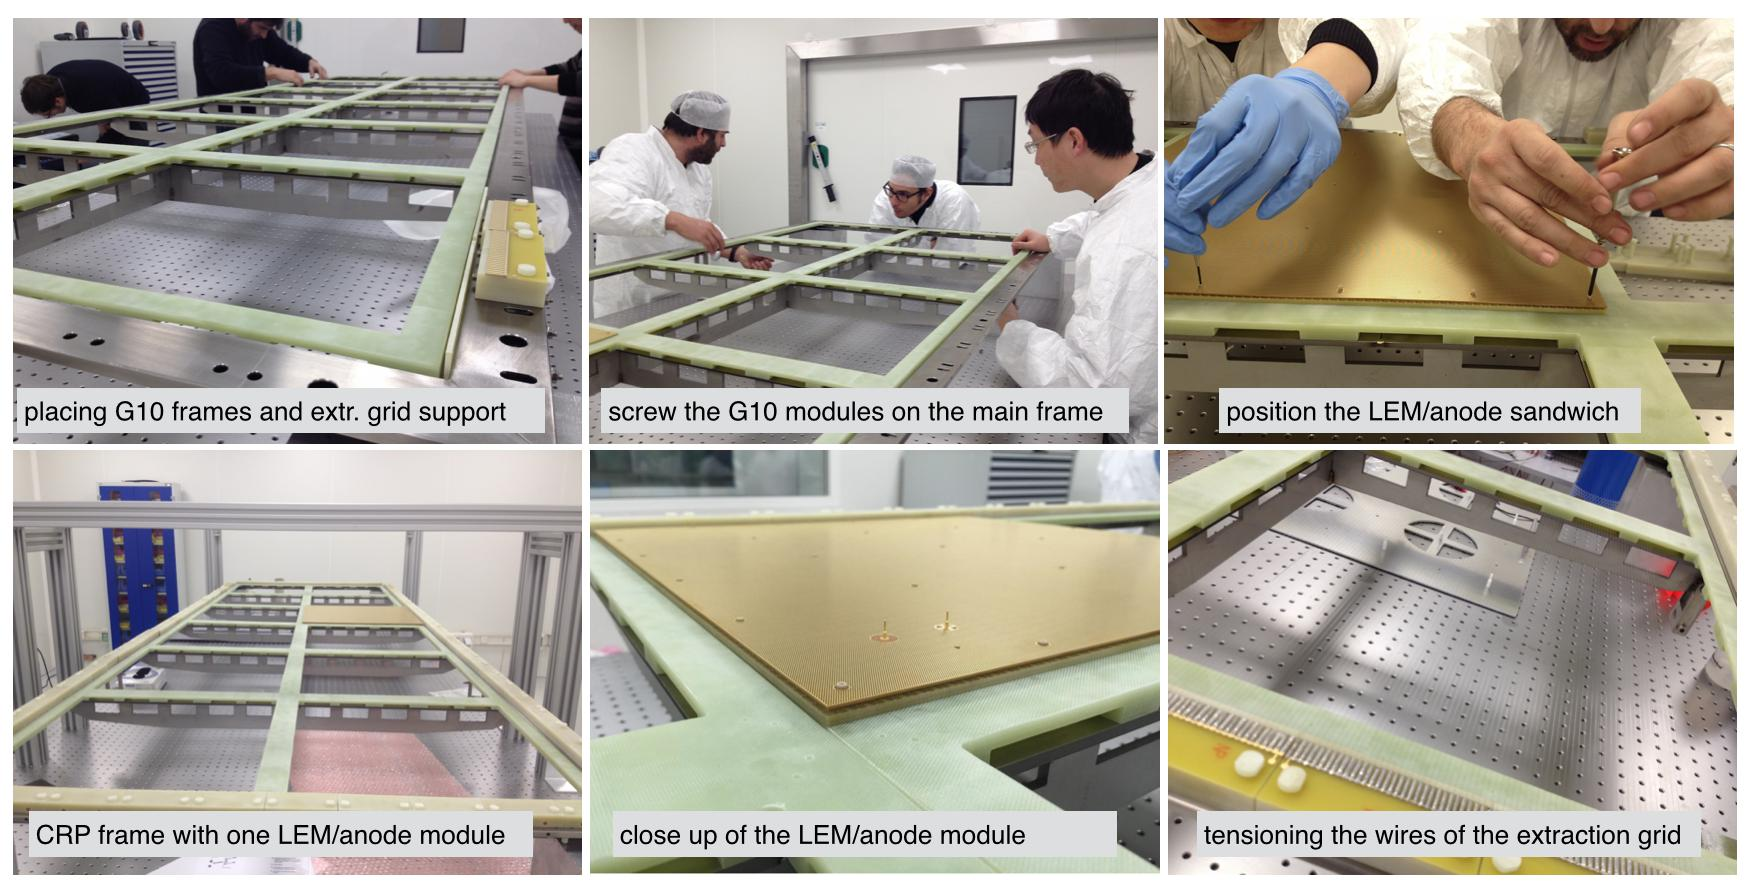
\includegraphics[width=\textwidth]{311_CRP_assembly}  
\end{cdrfigure}
